\chapter{Virtualisation} % mal écrit mais je pose les idées comme ça pour l'instant

Afin de vérifier que les actions de l'administrateur réseau ont des conséquences. Nous devions mettre en place de la virtualisation car on n'avait pas à disposition un réseau physique sur lequel faire nos redirection vers un trou noir.

La virtualisation est une donc part très importante du projet. En effet, cela nous a permis de créer un environnement virtuel adéquat pour l'exécution de notre logiciel dans des conditions optimales.
Cependant, il faut tout de même travailler cette mise en place et réfléchir à une bonne topologie. Heureusement, le client nous aura fourni les moyens nécessaires pour exécuter cette tâches.

\section{Pré-requis}
Avant de s'atteler à la virtualisation et le lancement de machines virtuelles, il nous faut un certains nombres d'outils qui nous seront utiles par la suite. Nous allons donc détailler chacun d'entre eux.

\subsubsection{Topologies}
Voici la topologie que l'on a réalisé grâce à la proposition de notre client. Pour cela, on a suivi son sujet de \href{http://dept-info.labri.fr/~magoni/rvep/TD-RTBHR/TD-RTBHR.pdf}{TP}.

\begin{figure}
    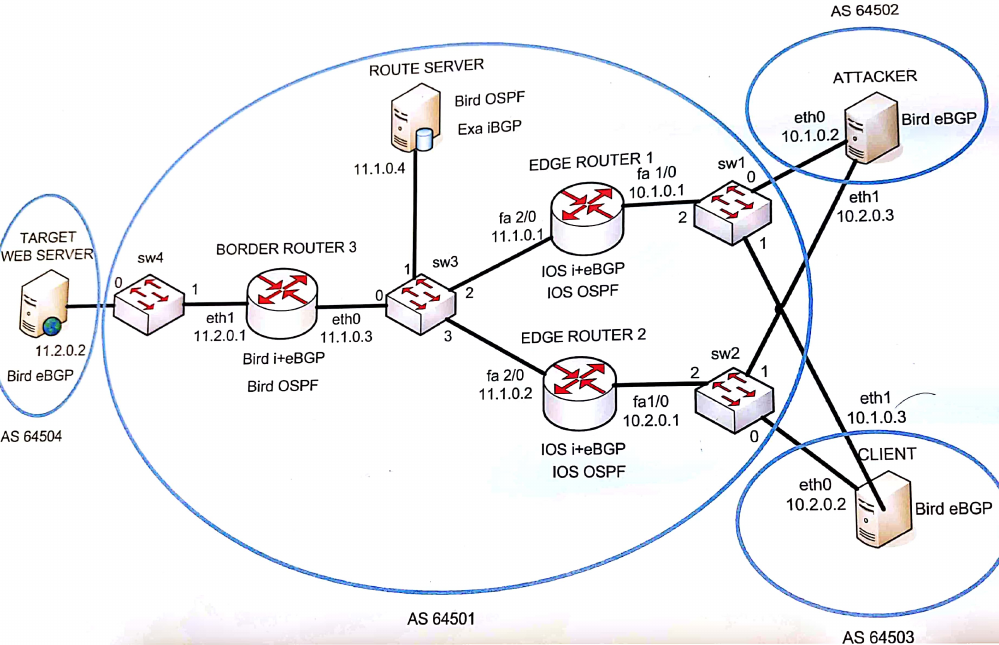
\includegraphics[width=\textwidth]{topologie.png}
    \caption{Topologie}
    \label{fig:topo}
\end{figure}

% image topo + explications
Nous avons donc cinq machines différentes pour notre simulation :
\begin{itemize}
    \item [\textbf{attacker}] : la machine attaquante,
    \item [\textbf{target}] : le serveur cible,
    \item [\textbf{client}] : une machine client quelconque,
    \item [\textbf{border-router}] : le routeur de frontière,
    \item [\textbf{route-server}] : le serveur de route où sera lancé notre projet
\end{itemize}
Chaque machine possédera sa propre configuration qu'on importera par la suite.
\subsubsection{Nemu}
Comme expliqué dans l'Analyse de l'existant, c'est un environnement de réseaux virtuels distribués gérant des machines virtuelles de type QEmu. Il nous servira à générer et à relier les différentes machines entre elles, via un script préalablement établi.

\subsubsection{Dynamips}
Dynamips est un émulateur de routeur de type Cisco. Grâce a une image Cisco, fourni par notre client, il nous a permis de créer les images de deux routeurs Cisco. Avant de les lancer, il faut obtenir l'idle-pc avec un count le plus élevé. En effet, cela permettra aux routeurs de limiter leur utilisation du processeur et ainsi gagner en fluidité.

\subsubsection{Bird}
Bird est un logiciel open source implémentant l'envoi de paquet IP sur le réseau pour des machines de type Unix. Il nous permettra donc de simuler le trafic sur notre petit réseau, ainsi que de générer les deux protocoles principaux iBGP et eBGP. Chaque machine possédera sa propre configuration Bird qu'on importera par la suite.

\subsubsection{Debian}
Il nous faudra bien évidemment un système d'exploitation sur toutes nos machines et celles-ci posséderont donc Debian 8.

\subsubsection{ExaBGP}
Nous permettra donc de diffuser les routes sur le réseaux via BGP.

\section{Configuration des Machines Virtuelles}

Dans un premier temps, nous lançons le script \verb+dyna.sh+, permettant l'initialisation des deux routeurs cisco.
Une fois cela fait, nous pouvons lancer Nemu avec un script préalablement rédigé par nos soins décrivant la topologie de la simulation.
Cinq fenêtres vont donc s'ouvrir, une pour chaque machine. Leur nom est inscrit dans la barre de titre située au dessus de chaque fenêtre.
Une fois les fenêtres chargées, une page de login s'affiche. Nous nous connecterons dessus en tant que \verb+root+.

Une fois connecté, il faut configurer les interfaces réseaux. Les fichiers de configuration ont préalablement été fait, il ne reste plus qu'à les importer directement sur les machines.
Toujours penser à redémarrer le service pour que la nouvelle interface soit prise en compte.

On pourra tester la connectivité à l'aide de \verb+ping+ entre les différentes machines.
Si cela est concluant, nous pouvons passer à la suite.

Ensuite, il faut installer Bird sur toutes les machines sauf le \textbf{route-server}, et importer les fichiers de configuration préalablement rédigés également.

On pourra vérifier le bon fonctionnement de Bird avec la commande \verb+birdc sh proto+, qui affichera une liste des protocoles en cours.

Enfin, sur le \textbf{route-server}, il nous faut donc installer ExaBGP via \verb+pip+ de Python.
Une fois cela fait, il faudra importer les fichiers de configuration, qui ont aussi été rédigés au préalables.
Il faudra bien évidemment démarrer le service via la commande \verb+systemctl start exabgp+.

On peut voir le bon lancement d'ExaBGP avec la commande \verb+systemctl status exabgp+. En effet, nous pourrons effectivement voir si le service est actif ou non.

\section{Lancement du projet}

Sur le \textbf{route-server}, il faut importer le projet, de la même manière que l'on a importé les fichiers de configuration pour les différents modules.
Avant de lancer le projet, il nous faut un environnement virtuel, qu'il faudra installer.
Une fois l'environnement virtuel lancé, il faut installer tous les paquages nécessaire au bon déroulement du projet.
Dans ce terminal, nous allons lancé notre API.
Dans un autre terminal, nous activons l'environnement virtuel et nous lançons donc le frontend. Un lien s'affiche, nous n'avons plus qu'à cliquer dessus. Le navigateur va donc s'ouvrir sur une page d'administration.
Il ne reste plus qu'à se connecter et nous pouvons enfin découvrir notre interface utilisateur.

\section{Tests}
Sur la machine \textbf{client} et la machine \textbf{attacker}, on effectue un ping vers la machine \textbf{target}.
Sur notre interface utilisateur, nous allons entrer l'ip de la machine attaquant et la rediriger vers une adresse fictive. Nous n'avons pas besoin d'entrer de communauté.
Après l'envoi du formulaire, le ping de la machine attaquant est stoppé alors que celui de la machine cliente continue de tourner.
La cible est donc protégée.
Nous allons maintenant désactiver la route, et nous voyons bien qu'elle est toujours présente dans la liste des routes créées. Le ping a donc repris.
Nous pouvons donc voir que de ce point de vue là, notre projet fonctionne correctement.

%tester les commandes
%on peut verifier avec le status exabgp -l
